\subsection{SURF}
SURF, ligesom SIFT, er en fuldstændig løsning, til at finde og beskrive blobs, som består af en detektor og en deskriptor. I forhold til SIFT, har SURF den fordel, at den beregningsmæssigt kan optimeres til at være hurtigere end SIFT, og metoden er mindre kompleks, fordi den består af færre beregningsskridt. SURF kan optimeres, igennem brug af integralbilleder[???].
\subsubsection{Detector}
\begin{figure}[H]
    \centering
    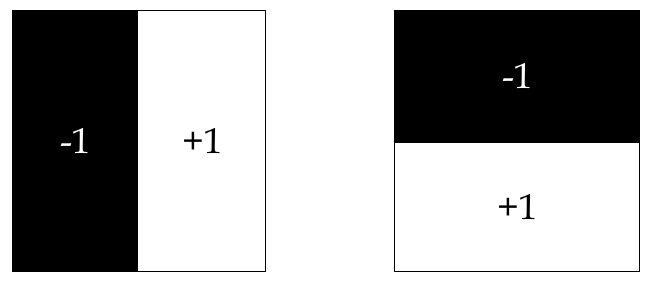
\includegraphics[width=0.65\textwidth]{fig/haarwavelet.png}
     \vspace{-1em}
    \begin{center}    
       \caption{\textcolor{gray}{\footnotesize \textit{ }}}
    \label{fig:difference}
     \end{center}
     \vspace{-2.5em}
  \end{figure} \noindent

SURF gør brug af Haar-wavelet, både i detektoren og deskriptoren. Haar-wavelet er et boks-filter, med størrelse nxn, hvor halvdelen af alle indgangene er +1 og den anden halvdel er -1.


\subsubsection{Deskriptor}
SURF deskriptoren producerer features, der består af 64 indgange. Den kan beskrives stringent, ligesom (26). Som beskrevet i SURF papiret af Tuytelaars et. al[??], er tilfældet ofte, at der ikke er brug for rotationsinvarians. En variant af SURF, der ikke er rotationsinvariant, kaldes Upright-SURF (U-SURF). Tuytelaars et. al garanterer dog rotationsinvarians i U-SURF, i op til $\pm 15^{\circ}$. SURF er implementeret, fremfor U-SURF, da enkelte af billederne har stor grad (ca. $15^{\circ}$) af rotation. Rotationen forekommer i billeder, der er taget lige efter, at dronen har vendt og kan ses på figur 15.
\\
\\
SURF deskriptoren samler data omkring interssepunktet, med et dataindsamlingvindue der har størrelse $20 \sigma$. Vinduet skal orienters, ifht. den $\theta$ værdi, der er udregnet i detektoren. Billedet vendes, ved, at vende hele billedet, ved brug af ligning \eqref{rotaionmatrix}, og danne et integralbillede udfra det nye billede (Dette skridt er omkostningsfuldt, og der vil senere blive diskuteret optimeringer).
\\
\\
Dataindsamlingsvinduet er nu roteret og centreret omkring interessepunktet. Herefter skal vinduet deles op i 4x4 regioner, hver bestående af 5x5 punkter, der har ens afstand mellem sig - her er ikke blevet lavet subpixel-optimeringen, så hvis $\frac{20\sigma}{4}$ ikke er deleligt med 5, bliver der rundet ned.
\\
\\
Herefter skal Haar-wavelet responset udreges, i x og y retningen ($dx, dy$, respektivt). Haar-wavelet skal udregnes for alle punkter i 5x5 felterne. Størrelsen på Haar-wavelet filteret, er $2\sigma$. Disse værdier skal smoothes med et Gaussfilter, hvor $\sigma_{Gauss} = 3.3\sigma_{point}$.
\\
\\
For her af de 16 4x4 regioner, udregnes: $v_i = \sum d_x, \sum d_y, \sum |d_y|, \sum |d_y|$, hvor $v_i$ er beregningerne, for den $i$'ende region. Der laves en vektor, hvor alle værdierne indgange i $v$ sættes efter hinanden. Dette giver en $16 \cdot 4 = 64$ indgange stor vektor. Slutteligt, laves vektoren om til en enhedsvektor.
